\documentclass{article}
\usepackage[a4paper]{geometry}
\usepackage{authblk}
\usepackage{natbib}
\usepackage{graphicx}
\setcitestyle{authoryear,open={(},close={)}}
\author[1]{Bastian Schiffthaler <bastian.schiffthaler@umu.se>}
\author[2]{Nicolas Delhomme}
\author[4]{Carolina Bernhardsson}
\author[3]{Jerry Jenkins}
\author[1]{Stefan Jansson}
\author[4]{P{\"a}r Ingvarsson}
\author[3]{Jeremy Schmutz}
\author[1]{Nathaniel Street}
\affil[1]{Ume\aa\ University, dept. of Plant Physiology, Ume{\aa}, Sweden}
\affil[2]{Swedish University of Agricultural Sciences, dept. of Plant Physiology, Ume{\aa}, Sweden}
\affil[3]{HudsonAlpha Institute for Biotechnology, Huntsville Al, USA}
\affil[4]{Swedish University of Agricultural Sciences, dept. of Plant Biology and Forest Genetics, Uppsala, Sweden}
\title{An Improved Genome Assembly of the European Aspen {\it Populus tremula}}
\date{}
\begin{document}
\maketitle

\section{Introduction}
The {\it Populus} genus consists of about 30 species, which are commonly found in the Northern Hemisphere. They are an important model system for forest tree research, an ecological pioneer species, and of high commercial interest due to their rapid growth and ease of propagation \citep{stettler1996biology}.\\
The genome assembly of the European aspen {\it Populus tremula} \citep{LinE10970} proved difficult for a short-read based strategy due to high genomic variation. As a consequence, the fragmented sequence is impeding studies that benefit from highly contiguous data, particularly genome-wide association studies (GWAS) and comparative genomics.\\  
Here we present an updated assembly based on long-read sequences, optical mapping and genetic mapping. This assembly - henceforth referred to as {\it Potra} V2 - is assembled into 19 contiguous chromosomes which provides a powerful tool for future association studies.\\
The genome sequence and any feature files are available from the PopGenIE resource \citep{sjodin2009populus}.\\

\section{Results and Discussion}
\subsection{Genome Assembly}
% First round fixing  : 1977238
% Second round fixing :  144040
% Pilon fix: 18548 continuity breaks
% 310208 SNPs, 5854 Ambiguous, 498309 INS for 1020777 bases, 83368 DEL for 650757 bases
% Basic stats
The {\it P. tremula} genome assembled into 19 chromosomes and 1582 scaffolds with a combined length of 408834716bp. Aligning \~95M Illumina reads (about 20x coverage) yields a 96.4\% (97.77\% in V1) map percentage with 94.19\% (92.33\% in V1) of these maps in proper pairs. The increase in proper pairs and a decrease in overall mapping reflects our expectation from an assembly with higher contiguity but lower per-base accuracy. Table \ref{T1} provides additional summary statistics for the raw assembly.\\ 
\begin{table}
\caption{Summary statistics for {\it P. tremula} version 2.}
\label{T1}
\begin{center}
\begin{tabular}{|c|c|c|}
\hline
Statistic & Potra01 & Potra02 \\
\# contigs (>= 0 bp) & 204318 & 1601 \\
\# contigs (>= 1000 bp) & 31632 & 1584 \\
\# contigs (>= 5000 bp) & 7267 & 1339 \\
\# contigs (>= 10000 bp) & 5151 & 986 \\
\# contigs (>= 25000 bp) & 3209 & 491 \\
\# contigs (>= 50000 bp) & 1789 & 255 \\
Total length (>= 0 bp) & 386236512 & 408834716 \\
Total length (>= 1000 bp) & 328536064 & 408824553 \\
Total length (>= 5000 bp) & 277117215 & 407999588 \\
Total length (>= 10000 bp) & 262322877 & 405364617 \\
Total length (>= 25000 bp) & 231504505 & 397478443 \\
Total length (>= 50000 bp) & 180499961 & 389097052 \\
\# contigs & 12044 & 1489 \\
Largest contig & 418873 & 53234430 \\
Total length & 294670244 & 408605800 \\
GC (\%) & 33.56 & 33.87 \\
N50 & 69979 & 16928776 \\
N75 & 29987 & 13637973 \\
L50 & 1227 & 9 \\
L75 & 2826 & 15 \\
\# N's per 100 kbp & 5428.58 & 6573.91 \\
Reads aligned (\%) & 97.77\% & 96.40\% \\
Reads properly paired (\%) & 92.33\% & 94.19\% \\
\hline
\end{tabular}
\end{center}
\end{table}\\
% BUSCO
Analysis of the genome using BUSCO \citep{simao2015busco} with the \verb|embryophyta_odb10| ortholog set showed 96.8\% (96.8\% in V1) complete BUSCOs, of which 81.7\% (82.5\% in V1) were single copy and 15.1\% (14.3\% in V1) duplicated. The first version of the assembly scored better in duplication and missing BUSCOs. Detailed values follow in table \ref{T2}.\\

\begin{table}
\caption{BUSCO genome statistics for both assemblies.}
\label{T2}
\begin{center}
\begin{tabular}{|c|c|c|}
\hline
BUSCO & Potra01 & Potra02 \\
Complete & 96.8\% & 96.8\% \\
Single Copy & 82.5\% & 81.7\% \\
Duplicated & 14.3\% & 15.1\% \\
Fragmented & 1.5\% & 0.9\% \\
Missing & 1.7\% & 2.3\% \\
\hline
\end{tabular}
\end{center}
\end{table}

% LTRi
The long terminal repeat (LTR) index for the assembly \citep{10.1093/nar/gky730} is 6.65, with 1.42\% of intact LTRs 20.66\% of total LTRs. This LTR index indicates a high-quality draft assembly comparable to apple v1.0 or cacao v1.0.\\
% SV PB aligments to median coverage of 40 (V1) and 44 (V2) so alignment quality is not a huge factor
Analysis of structural variation in both genomes showed fewer overall variants in PotraV2, but a higher rate of insertions and inversions. The extremely high number of detected translocation events in PotraV1 is likely due to the overall fragmentation of the genome.\\
\begin{table}
\caption{Structural variants called after auto-alignment}
\label{T4}
\begin{center}
\begin{tabular}{|c|c|c|}
\hline
Variant & Potra01 & Potra02 \\
Translocation & 126172 & 23920 \\
Copy Number Variant & 5284 & 1332 \\
Deletion & 44770 & 35290 \\
Insertion & 22848 & 36864 \\
Inversion & 25 & 108 \\
Split & 965 & 853 \\
\hline
\end{tabular}
\end{center}
\end{table}

Synteny alignments between V1 and V2 showed that 59.6\% of genomic regions on chromosomes (55.1\% when including scaffolds) in V2 have a corresponding V1 alignment. The extent of the difference in these assemblies is suprising, especially given the high mapping rates of genomic shotgun sequence. It is plausible that the regions that are missed are comprised of sequence that is traditionally problematic for short-read assemblies, e.g.: repeats. Figure \ref{F1} shows a visual representation of the synteny alignments for the 19 chromosomes in V2. 

\begin{figure}
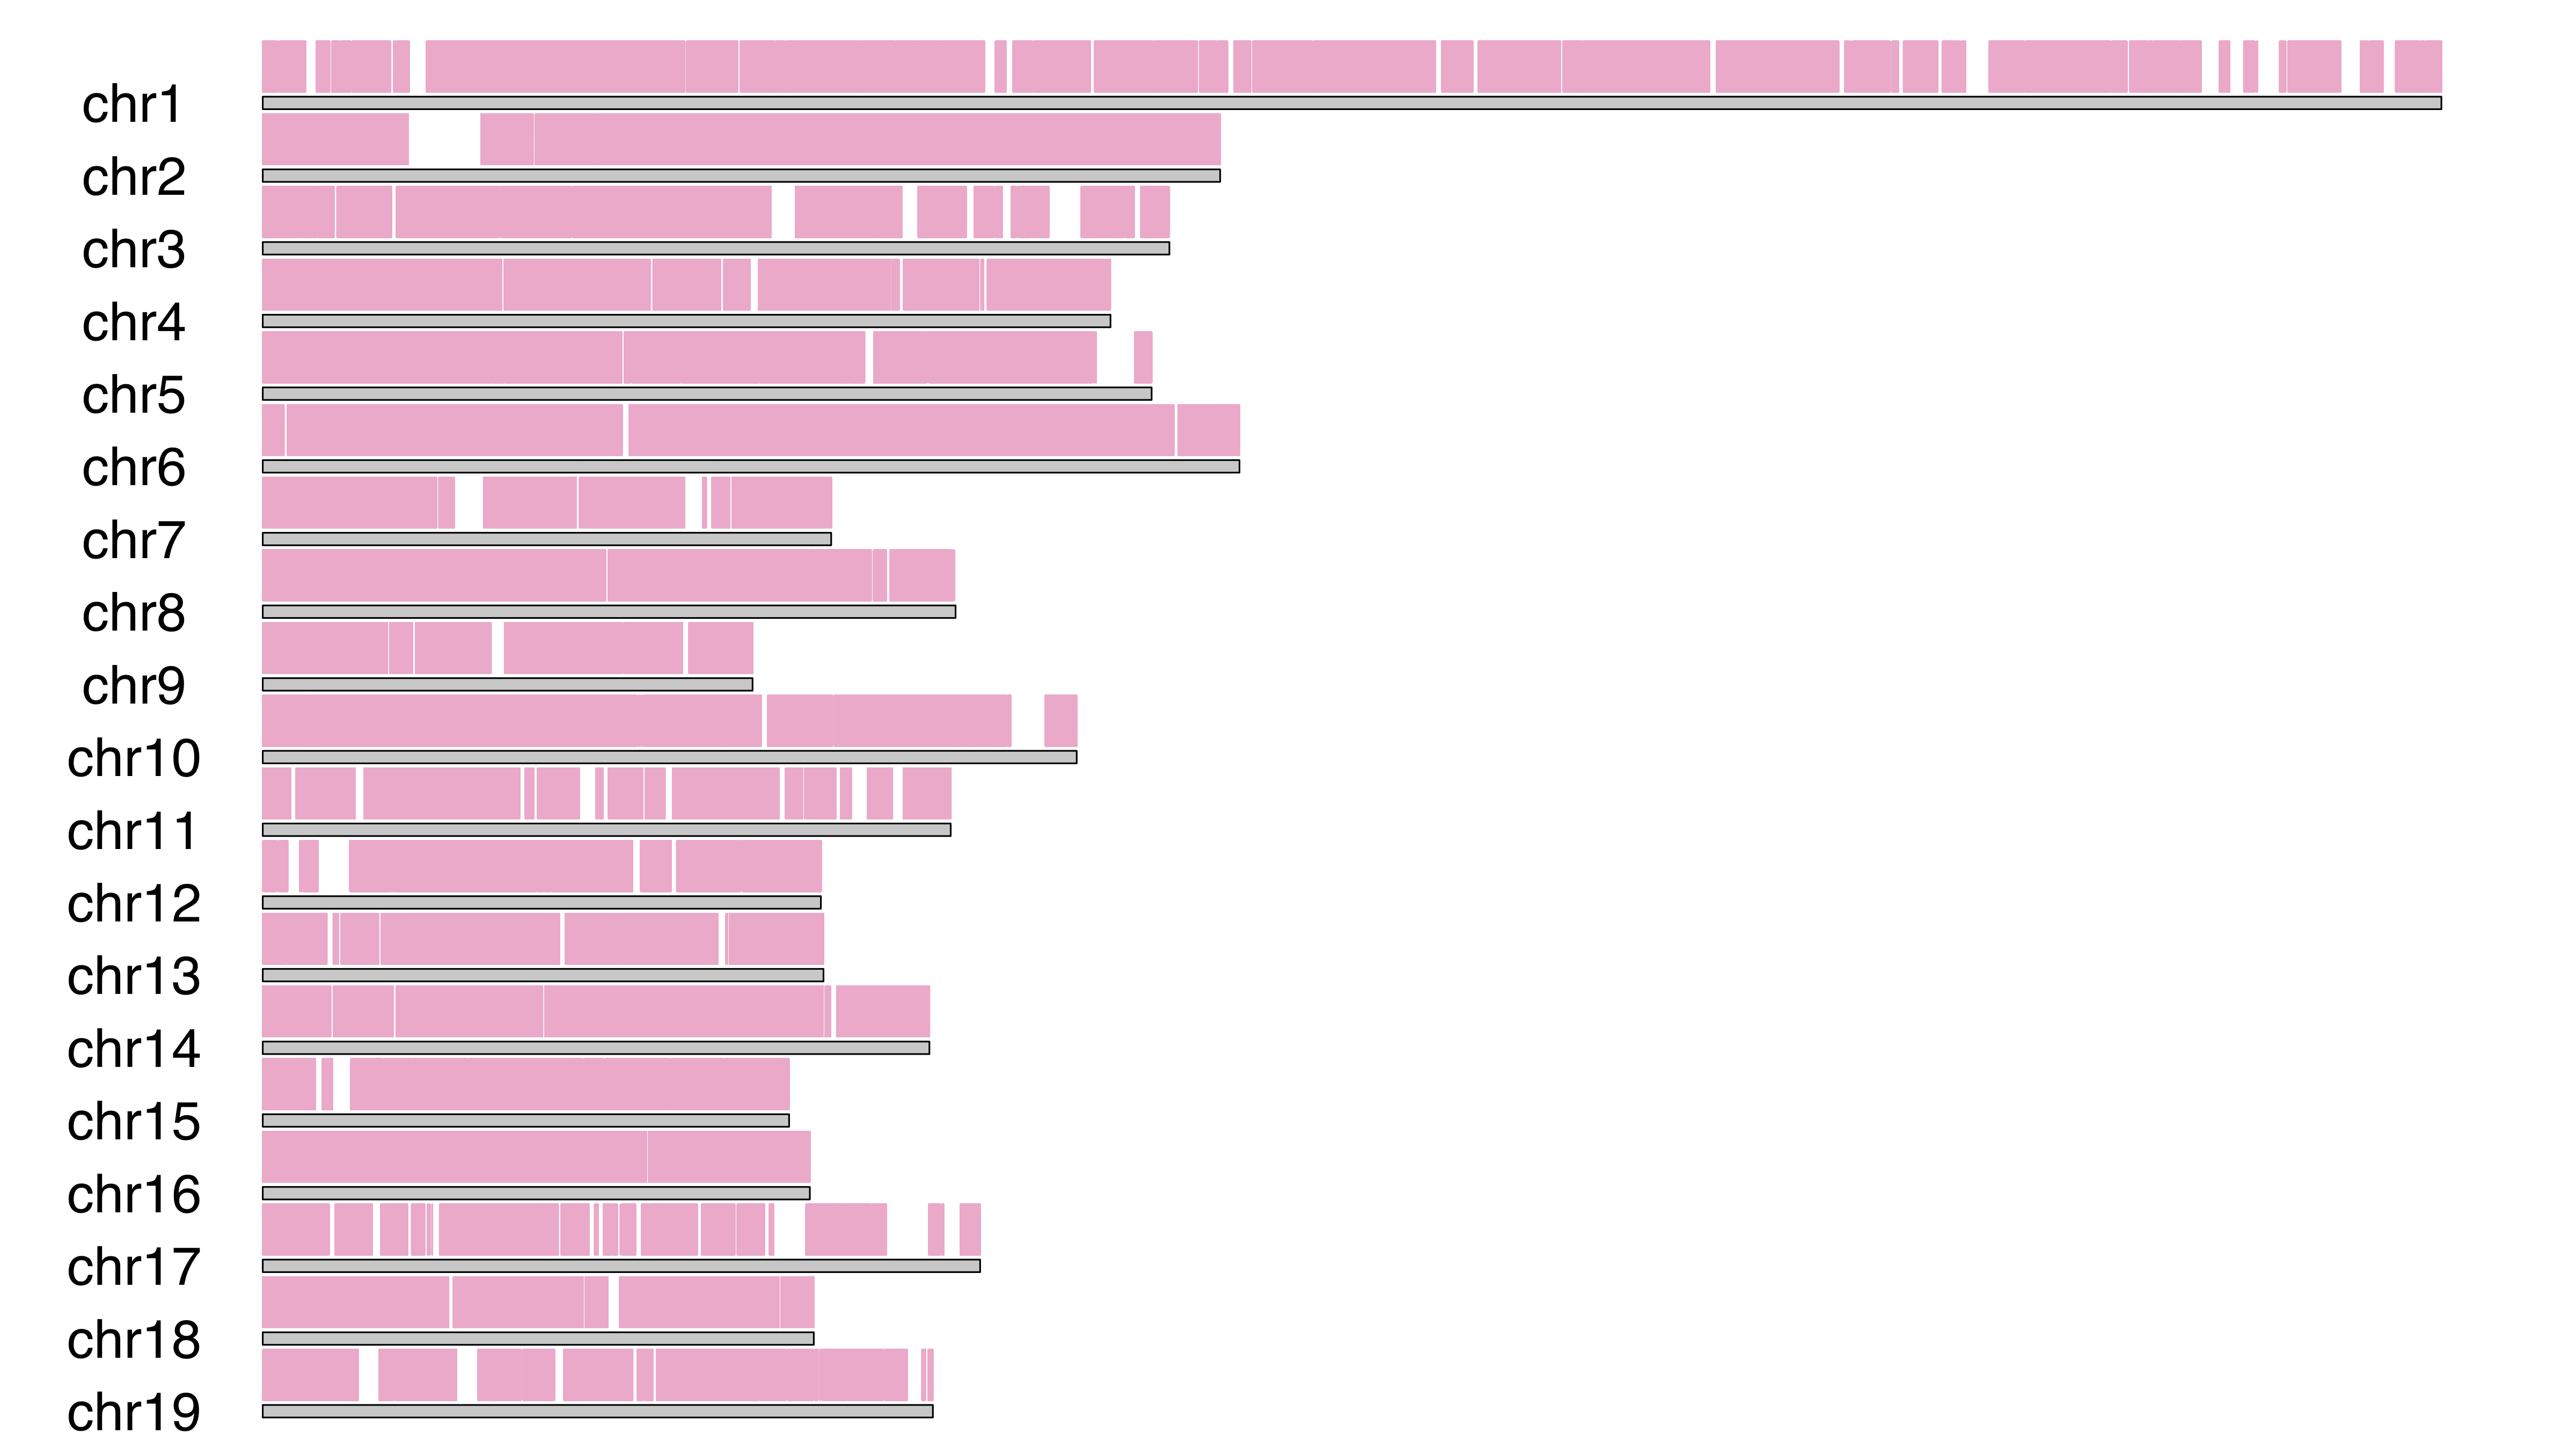
\includegraphics[width=\textwidth]{pv1synteny.png}
\label{F1}
\caption{Synteny alignment of the version 1 assembly to the version 2 assembly. Blocks with a highly similar synteny alignment are shaded red.}
\end{figure}

\subsection{Gene annotation}
% Basic stats
We identified in total 39894 gene models, 37184 of which on chromosomes and 2710 on scaffolds. In total, we detected 77949 transcripts, 73765 on chromosomes and 4184 on scaffolds (\~1.95 transcripts per gene). We found functional annotations for 73765 transcripts in 37184 genes.\\
% BUSCO trans
Analysis of the predicted transcripts using BUSCO with the \verb|embryophyta_odb10| ortholog set showed 98.1\% (96.8\% in V1) complete BUSCOs, of which 35.7\% (30.2\% in V1) were single copy and 62.4\% (66.6\% in V1) duplicated. Version 2 of the assembly performed slightly better in complete and single-copy BUSCOs. Detailed values follow in table \ref{T3}.\\

\begin{table}
\caption{BUSCO transcript statistics for both assemblies.}
\label{T3}
\begin{center}
\begin{tabular}{|c|c|c|}
\hline
BUSCO & Potra01 & Potra02 \\
Complete & 96.8\% & 98.1\% \\
Single Copy & 30.2\% & 35.7\% \\
Duplicated & 66.6\% & 62.4\% \\
Fragmented & 2.3\% & 0.9\% \\
Missing & 0.9\% & 1.0\% \\
\hline
\end{tabular}
\end{center}
\end{table}

\section{Materials and Methods}

If not otherwise specified, we omitted irrelevant arguments (s.a. file paths, parallelism) from command lines for the sake of clarity.\\
If no arguments are specified, we did not make any changes to the defaults.\\
Unless otherwise specified, we aligned genomic data with BWA mem v0.7.8-r455 \citep{li2013aligning} and RNA-Seq data with STAR v2.6.1d \citep{dobin2013star}.\\
All scripts and config files can be found in the Git repository: https://github.com/bschiffthaler/aspen-v2\\

\subsection{Data}
Unless otherwise specified Science for Life Laboratory in Stockholm generated all sequence data.\\
For genome assembly and correction, we generated two libraries:\\
\begin{itemize}
%PB 3581635 reads
\item ``PacBio data'': 28874072954 bases (filtered subreads, \~60x coverage), Pacific Biosciences on the RSII platform. ENA: TBD
\item ``Illumina data'': 108353739802 bases (\~226x coverage), Illumina HiSeq2500. ENA: TBD
\end{itemize}
We also collected several RNA-Seq datasets for use in the genome annotation:\\
\begin{itemize}
\item ``AspWood'' \citep{sundell2017aspwood} (ENA: ERP016242)
\item ``Sex'' \citep{robinson2014populus} (ENA: ERP002471)
\item ``SwAsp'' \citep{mahler2017gene} (ENA: ERP014886)
\item ``Assembly version 1 tissue atlas'' \citep{LinE10970} (ENA: PRJEB23585)
\item ``Xylem/Leaf'' \citep{LinE10970} (ENA: PRJEB23585)
\item ``Leaf Development'' (Unpublished data, sequenced by BGI Genomics)
\end{itemize}

\subsection{Assembly}
Initially, we assembled the genome using FALCON v0.3 \citep{chin2016phased}. We include the FALCON config file in the Git repository. Subsequently, we aligned all the Illumina data to the initial assembly and used in-house scripts to correct homozygous SNPs and small INDEL issues. We then aligned the Illumina data to the fixed assembly and repeated the first round of fixing. For a third and final round of fixing, we used the Illumina data as input to Pilon \citep{walker2014pilon} v2.11-1.18 to correct assembly issues per scaffold.\\
In order to reduce the presence of split haplotypes, we used HaploMerger2 \citep{huang2017haplomerger2} (retrieved: 2015-11-06). We include all HaploMerger2 scripts in the Git repository.\\
We subsequently created an optical map of the genome in collaboration with BioNano genomics, which we utilized to further scaffold and orient our current assembly.\\
Finally, we used the high-density genetic linkage map from \cite{apuli2019constructing} as input to ALLMAPS \citep{tang2015allmaps} to place the scaffolds into chromosomes.\\

\subsection{Transcriptome Assembly}
To provide evidences for the gene annotation process, we used trinity \citep{grabherr2011trinity} to assemble the transcriptome of five RNA-Seq \citep{mortazavi2008mapping} datasets from Populus tremula. Four of the datasets had already been used for the annotation of the previous genome version \citep{LinE10970}: exAtlas, exDiversity, Xylem.leaf and Leaf, while the fifth was derived from our AspWood resource \citep{sundell2017aspwood}. These five datasets are available from the ENA (https://ebi.ac.uk/ena) under the accessions PRJEB5040, PRJEB1790, PRJEB28867, PRJEB28866, PRJEB14593, respectively.
The reads were pre-processed as described in \cite{LinE10970} and Sundell \cite{sundell2017aspwood}. Briefly, the raw reads were filtered for rRNA using SortMeRNA \citep{kopylova2012sortmerna} version 2.1 and trimmed for adapter sequences and lower quality using Trimmomatic \citep{bolger2014trimmomatic} v0.39. The filtered reads were then assembled using trinity \citep{haas2013novo} version 2.8.4 using default settings. The resulting transcript fasta files were then used as evidence for Maker-P.

\subsection{Annotation}
We first collected a set of diverse RNA-Seq datasets from previous studies. These, we aligned to the genome using STAR in 2-pass mode. For the first pass, we used the following arguments:\\

\begin{verbatim}
STAR --outFilterType BySJout --outFilterMultimapNmax 20 --alignSJoverhangMin 8 \
  --alignSJDBoverhangMin 1 --outFilterMismatchNmax 999 \
  --outFilterMismatchNoverReadLmax 0.1 --alignIntronMin 20 \
  --alignIntronMax 20000 --alignMatesGapMax 5000 \
  --outSAMtype BAM SortedByCoordinate --chimOutType WithinBAM 
\end{verbatim}

For the second pass, we provided the splice junctions from the first pass as \verb|pass-1-SJ.out.tab| and used:\\

\begin{verbatim}
STAR --outFilterType BySJout --outFilterMultimapNmax 20 --alignSJoverhangMin 8 \
  --alignSJDBoverhangMin 1 --outFilterMismatchNmax 999 \
  --outFilterMismatchNoverReadLmax 0.1 --alignIntronMin 20 \
  --alignIntronMax 20000 --alignMatesGapMax 5000 \
  --outSAMtype BAM SortedByCoordinate --chimOutType WithinBAM \
  --limitSjdbInsertNsj 2000000 --sjdbFileChrStartEnd pass-1-SJ.out.tab  
\end{verbatim}

We then provided these alignments to BRAKER1 \citep{hoff2015braker1} along with protein sequences of version 1 of the assembly, running BRAKER1 in hybrid mode with arguments:\\

\begin{verbatim}
braker.pl --genome=genome.fa --prot_seq=protein.fa \
  --prg=gth --softmasking --AUGUSTUS_ab_initio
\end{verbatim}

In order to prepare the genome for annotation, we created a custom repeat library using RepeatModeler v1.0.11. We then concatenated the custom repeats with known repeats in {\it Viridiplantae} and the first assembly of the {\it P. tremula} genome. We masked the genome using RepeatMasker 4.0.8 \footnote{http://www.repeatmasker.org}.\\

We ran MAKER v2.31.10 \citep{campbell2014genome} on the masked genome in three passes. We include the MAKER config files in the Git repository. We used Trinity assemblies from all RNA-Seq datasets in conjunction with all transcripts from the v1 assembly as expressed sequence tag (EST) evidence. Further, we provided proteins from the v1 assembly and the v3.0 assembly of {\it P. trichocarpa} \citep{tuskan2006genome} as protein evidence. In order to train AUGUSTUS v3.0.2 \citep{stanke2008using} and SNAP v2013-11-29 \citep{korf2004gene} we extracted confident predictions from the first run of MAKER using \verb|maker2zff| from the MAKER suite and \verb|zff2augustus_gbk.pl| from an external source\footnote{https://github.com/hyphaltip/genome-scripts/blob/master/gene\_prediction/zff2augustus\_gbk.pl}. We then proceeded with another round of MAKER including AUGUSTUS, SNAP and GeneMark-ES \citep{lomsadze2005gene}. We repeated this process of training AUGUSTUS and SNAP once more for a third and final round of MAKER.

\subsection{Functional Annotation}
We aligned the transcripts and protein-coding sequences retrieved from MAKER to the NCBI nt \citep{wheeler2006database} and UniRef90 \citep{uniprot2018uniprot} databases, respectively. For transcripts, we used Blast+ version 2.6.0+ with the non-default parameters: \verb|-evalue 1e-5| \citep{altschul1990basic}. For proteins, we used Diamond version 0.9.26 with default parameters \citep{buchfink2015fast}. We identified and extracted the sequences aligning solely to the NCBI nt database to complement the UniRef90 alignments using an ad-hoc script (available upon request). We then imported the resulting alignment files in Blast2GO \citep{gotz2008high} version 5.2. Finally, we used Blast2GO to generate the Gene Ontology (both GO and GO-Slim), PFAM \citep{el2018pfam} and KEGG \citep{kanehisa2000kegg} annotations. 

\subsection{Evaluation}
To calculate summary statistics of the assembly, we used QUAST v5.0.2 \citep{gurevich2013quast}, aligning a 20x coverage subset of the aspen V1 2x150 PE library data (ENA: PRJEB23581) to calculate mapping percentages.\\
We ran BUSCO v3.0.2 for both the genomic and transcript sequences. We retrieved the ``embryophyta\_odb10'' dataset from {https://busco.ezlab.org/}.\\

\subsection{Figures and Data Processing}
We used the \verb|karyoplotR| \citep{gel2017karyoploter} package for the R statistical framework \citep{team2019language} to generate karyoplots

\section{acknowledgements}
The work conducted by the U.S. Department of Energy Joint Genome Institute, a DOE Office of Science User Facility, is supported by the Office of Science of the U.S. Department of Energy under Contract No. DE-AC02-05CH11231. This work was supported by the Knut and Alice Wallenberg Foundation and the Umeå Plant Science Centre Berzelii Centre. N.R.S. was supported by the Trees and Crops for the Future project.

\bibliographystyle{main.bst}
\bibliography{main.bib} 

%%%%%%%%%%%% to attatch %%%%%%%%%%%%%
%% FALCON fc_run.cfg
%% Haplomerger cfg

\end{document}